%\documentclass[iop]{emulateapj}
%\documentclass[12pt, preprint]{emulateapj}
\documentclass[12pt, onecolumn]{emulateapj}

\usepackage{amsmath}
%\usepackage{bibtex}
%\bibliographystyle{unsrtnat}

\newcommand{\myemail}{aimalz@nyu.edu}
\newcommand{\textul}{\underline}

%\slugcomment{}

\shorttitle{Probabilistic inference of the Hubble parameter}
\shortauthors{Malz and Peters, et al.}

\begin{document}

\title{Probabilistic inference of the Hubble parameter}

\author{Alex Malz\altaffilmark{1}}
\author{Tina Peters\altaffilmark{2}}
\author{Lluis Galbany}
\author{Humna Awan}
\author{Anita Bahmanyar}
\author{Kara Ponder}
\altaffiltext{1}{Center for Cosmology and Particle Physics, Department of Physics,
  New York University, 4 Washington Pl., room 424, New York, NY 10003, USA}
 \altaffiltext{2}{Dunlap\dots}
\email{aimalz@nyu.edu}

\begin{abstract}
The BEAMS framework enables the use of probabilistic supernova classifications to estimate the Hubble parameter quantifying the relationship between distance and redshift over cosmic time.  This work extends BEAMS to replace high-confidence spectroscopic redshifts with probabilistic photometric redshifts, enabling inference of the Hubble parameter as a function of two probabilistic variables.  By combining posterior probabilities of supernova type and posterior probability distributions over host galaxy redshift, we infer a posterior probability distribution over the redshift-dependent Hubble parameter.  This work also produces a code that can be used for other regression problems in astrophysics that involve catalogs of two probabilistic variables.
\end{abstract}

\keywords{}

\section{Introduction}
\label{sec:intro}

\citet{kunz_bayesian_2007, kelly_flexible_2008}

\section{Methods}
\label{sec:meth}

This covers a complete sample, i.e. a catalog of all $N$ supernovae $ns$ in the universe, ever.  We'll add in the selection function later.

\vspace{1in}
\begin{figure}
\begin{center}
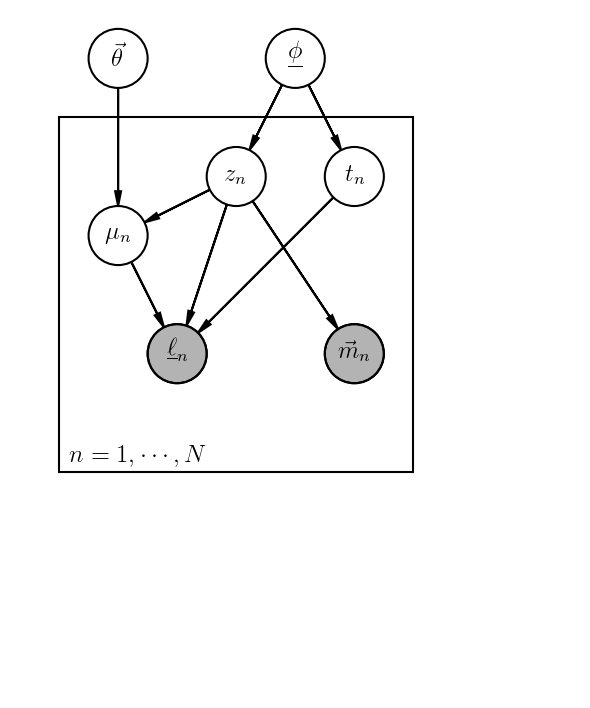
\includegraphics{Hubble-draft.png}
\caption{This directed acyclic graph corresponds to a probabilistic graphical model for our hierarchical inference of the Hubble parameter.  In this graph, all random variables are shown in circles, with observed variables shown in shaded circles.  The box indicates that there are $N$ copies of the relationships between boxed parameters, each independent of all others.  The hyperparameters we would like to infer are the cosmological parameters in $\vec{theta}$ and the supernova type-redshift distribution parameters comprising $\textul{\phi}$.  Drawn from functions of these hyperparameters are the distance moduli $\{\mu_{n}\}_{N}$, redshifts $\{z_{n}\}_{N}$, and supernova types $\{t_{n}\}_{N}$.  Here, we observe host galaxy colors $\{\vec{m}_{n}\}_{N}$ and multi-band supernova lightcurves $\{\textul{\ell}_{n}\}_{N}$, shown in shaded circles.}
\label{fig:pgm}
\end{center}
\end{figure}
\vspace{1in}

The goal here is to constrain the posterior distribution of the hyperparameters of interest given the data.

We first expand this in terms of Bayes' Rule.

\begin{align}
p(\vec{\theta}, \textul{\phi} | \{\textul{\ell}_{n}\}_{N}, \{\vec{m}_{n}\}_{N}) &\propto p(\vec{\theta}, \textul{\phi})\ p(\{\textul{\ell}_{n}\}_{N}, \{\vec{m}_{n}\}_{N} | \vec{\theta}, \textul{\phi})
\end{align}

Next, we invoke the independence of the supernova parameters and observations; the $n^{th}$ system's parameters and data are assumed to be independent of the $(n+1)^{th}$ system's parameters and data.

\begin{align}
p(\{\textul{\ell}_{n}\}_{N}, \{\vec{m}_{n}\}_{N} | \vec{\theta}, \textul{\phi}) &= \prod_{n}^{N}p(\textul{\ell}_{n}, \vec{m}_{n} | \vec{\theta}, \textul{\phi})
\end{align}

Next, we use marginalization of the latent variables, because we do not wish to estimate their values directly.

\begin{align}
p(\textul{\ell}_{n}, \vec{m}_{n} | \vec{\theta}, \textul{\phi}) &= \iiint p(\textul{\ell}_{n}, \vec{m}_{n} | \mu_{n}, z_{n}, t_{n})\ p(\mu_{n}, z_{n}, t_{n} | \vec{\theta}, \textul{\phi})\ d\mu_{n}\ dz_{n}\ dt_{n}
\end{align}

We note that the equation calls for likelihoods $\{p(\textul{\ell}_{n}, \vec{m}_{n} | \mu_{n}, z_{n}, t_{n})\}_{N}$, but what we have are interim posteriors $\{p(\mu_{n}, z_{n}, t_{n} | \textul{\ell}_{n}, \vec{m}_{n}, \vec{\theta}^{*}, \textul{\phi}^{*})\}_{N}$ for some interim priors $\vec{\theta}^{*}, \textul{\phi}^{*}$.  The interim priors represent the beliefs about the hyperparameters $\vec{\theta}$ and $\textul{\phi}$ that go into our calculation of the posteriors from the data; whether explicitly chosen (as in methods relying on a template library) or implicitly derived (as in methods relying on a training data set), the interim priors are always present in the calculation of posterior distributions from data.  We will thus have to transform the math to be in terms of quantities we actually have.  We do this by multiplying the likelihood by an inspired factor of unity, in terms of the interim posteriors.

\begin{align}
p(\textul{\ell}_{n}, \vec{m}_{n} | \mu_{n}, z_{n}, t_{n}) &= p(\textul{\ell}_{n}, \vec{m}_{n} | \mu_{n}, z_{n}, t_{n})\ \frac{p(\mu_{n}, z_{n}, t_{n} | \textul{\ell}_{n}, \vec{m}_{n}, \vec{\theta}^{*}, \textul{\phi}^{*})}{p(\mu_{n}, z_{n}, t_{n} | \textul{\ell}_{n}, \vec{m}_{n}, \vec{\theta}^{*}, \textul{\phi}^{*})}
\end{align}

We will expand the denominator of that factor of unity according to Bayes' Rule.

\begin{align}
p(\mu_{n}, z_{n}, t_{n}|\textul{\ell}_{n}, \vec{m}_{n}, \vec{\theta}^{*}, \textul{\phi}^{*}) &= \frac{p(\mu_{n}, z_{n}, t_{n} | \vec{\theta}^{*}, \textul{\phi}^{*})\ p(\textul{\ell}_{n}, \vec{m}_{n} | \mu_{n}, z_{n}, t_{n}, \vec{\theta}^{*}, \textul{\phi}^{*})}{p(\textul{\ell}_{n}, \vec{m}_{n} | \vec{\theta}^{*}, \textul{\phi}^{*})}
\end{align}

By the independence of different hierarchical levels in the probabilistic graphical model, we may split up the most daunting term in the above expression.

\begin{align}
p(\textul{\ell}_{n}, \vec{m}_{n} | \mu_{n}, z_{n}, t_{n}, \vec{\theta}^{*}, \textul{\phi}^{*}) &= p(\textul{\ell}_{n}, \vec{m}_{n} | \mu_{n}, z_{n}, t_{n})\ p(\textul{\ell}_{n}, \vec{m}_{n} | \vec{\theta}^{*}, \textul{\phi}^{*})
\end{align}

Noting the presence of $p(\textul{\ell}_{n}, \vec{m}_{n} | \mu_{n}, z_{n}, t_{n})$ and $p(\textul{\ell}_{n}, \vec{m}_{n} | \vec{\theta}^{*}, \textul{\phi}^{*})$ in both the numerator and denominator for $p(\textul{\ell}_{n}, \vec{m}_{n} | \mu_{n}, z_{n}, t_{n})$, we cancel the like terms to express the individual likelihoods in terms of known quantities.

\begin{align}
p(\textul{\ell}_{n}, \vec{m}_{n} | \mu_{n}, z_{n}, t_{n}) &= \frac{p(\mu_{n}, z_{n}, t_{n} | \textul{\ell}_{n}, \vec{m}_{n}, \vec{\theta}^{*}, \textul{\phi}^{*})}{p(\mu_{n}, z_{n}, t_{n} | \vec{\theta}^{*}, \textul{\phi}^{*})}
\end{align}

We are now ready to plug the individual likelihoods into the marginalization.

\begin{align}
p(\textul{\ell}_{n}, \vec{m}_{n} | \vec{\theta}, \textul{\phi}) &= \iiint p(\mu_{n}, z_{n}, t_{n} | \textul{\ell}_{n}, \vec{m}_{n}, \vec{\theta}^{*}, \textul{\phi}^{*})\ \frac{p(\mu_{n}, z_{n}, t_{n} | \vec{\theta}, \textul{\phi})}{p(\mu_{n}, z_{n}, t_{n} | \vec{\theta}^{*}, \textul{\phi}^{*})}\ d\mu_{n}\ dz_{n}\ dt_{n}
\end{align}

Now we can plug the marginalization back into the product.

\begin{align}
p(\{\textul{\ell}_{n}, \vec{m}_{n}\}_{N} | \vec{\theta}, \textul{\phi}) &= \prod_{n}^{N}\ \iiint p(\mu_{n}, z_{n}, t_{n} | \textul{\ell}_{n}, \vec{m}_{n}, \vec{\theta}^{*}, \textul{\phi}^{*})\ \frac{p(\mu_{n}, z_{n}, t_{n} | \vec{\theta}, \textul{\phi})}{p(\mu_{n}, z_{n}, t_{n} | \vec{\theta}^{*}, \textul{\phi}^{*})}\ d\mu_{n}\ dz_{n}\ dt_{n}
\end{align}

And finally, we can plug the product back into Bayes' Rule.

\begin{align}
p(\vec{\theta}, \textul{\phi} | \{\textul{\ell}_{n}, \vec{m}_{n}\}_{N}) &\propto p(\vec{\theta}, \textul{\phi})\ \prod_{n}^{N}\ \iiint p(\mu_{n}, z_{n}, t_{n} | \textul{\ell}_{n}, \vec{m}_{n}, \vec{\theta}^{*}, \textul{\phi}^{*})\ \frac{p(\mu_{n}, z_{n}, t_{n} | \vec{\theta}, \textul{\phi})}{p(\mu_{n}, z_{n}, t_{n} | \vec{\theta}^{*}, \textul{\phi}^{*})}\ d\mu_{n}\ dz_{n}\ dt_{n}
\end{align}

This is the posterior we will attempt to sample!

\section{Mock Data}
\label{sec:data}

In order to simulate a mock dataset of three-dimensional posterior distributions $\{p(\mu_{n}, z_{n}, t_{n} | \textul{\ell}_{n}, \vec{m}_{n}, \vec{\theta}^{*}, \textul{\phi}^{*})\}_{N}$ over supernova type, redshift, and distance modulus, we will have to employ a forward model.

Since we are aiming to construct posteriors, we know from Bayes' Rule that they will take the form of Eq. \ref{eq:mockBayes}.

\begin{align}
\label{eq:mockBayes}
p(\mu_{n}, z_{n}, t_{n} | \textul{\ell}_{n}, \vec{m}_{n}, \vec{\theta}^{*}, \textul{\phi}^{*}) &\propto p(\textul{\ell}_{n}, \vec{m}_{n} | \mu_{n}, z_{n}, t_{n}, \vec{\theta}^{*}, \textul{\phi}^{*})\ p(\mu_{n}, z_{n}, t_{n} | \vec{\theta}^{*}, \textul{\phi}^{*})
\end{align}

We will discuss the two terms separately, starting with the second.  According to Fig. \ref{fig:pgm}, we have Eq. \ref{eq:second}.

\begin{align}
\label{eq:second}
p(\mu_{n}, z_{n}, t_{n} | \vec{\theta}^{*}, \textul{\phi}^{*}) &= p(\mu_{n} | z_{n}, \vec{\theta}^{*})\ p(z_{n}, t_{n} | \textul{\phi}^{*})
\end{align}

The first term of Eq. \ref{eq:mockBayes} may easily be reduced to $p(\textul{\ell}_{n}, \vec{m}_{n} | \mu_{n}, z_{n}, t_{n})$, as there is no direct dependence of the data on the hyperparameters is nontrivial.  Fig. \ref{fig:pgm} tells us how to break it up, resulting in Eq. \ref{eq:first}.

\begin{align}
\label{eq:first}
p(\textul{\ell}_{n}, \vec{m}_{n} | \mu_{n}, z_{n}, t_{n}) &= p(\textul{\ell}_{n} | \mu_{n}, z_{n}, t_{n})\ p(\vec{m}_{n} | z_{n})
\end{align}

There are many ways to formulate the various terms in Eqs. \ref{eq:first} and \ref{eq:second}, but we will restrict ourselves to the simplest version for now, outlined below in Sec. \ref{sec:choices}.  

\subsection{Model Specifics}
\label{sec:choices}

We establish the following domains for the latent variables $\{\mu_{n}\}$, $\{z_{n}\}$, and $\{t_{n}\}$.  There are $T$ possible values $\tau$ for $t$, defining a discrete space of types.  $z$ and $\mu$ are defined in binned spaces with $Z$ bins $\zeta$ of widths $\vec{\Delta}_{z}$ and $D$ bins $\nu$ of widths $\vec{\Delta}_{\mu}$ respectively.  

$\textul{\phi}$ may then be represented as a $T\times Z$ two-dimensional array satisfying $\sum_{\tau}^{T}\textul{\phi}\cdot\vec{\Delta}_{z}=1$, i.e. $p(z_{\zeta}, t_{\tau} | \textul{\phi}) \equiv \phi_{\zeta\tau}$.  For simplicity, we shall state that $\vec{\theta}\equiv H_{0}$, assuming all other cosmological parameters are perfectly known and forbidding redshift evolution.  Rather than writing the form of the distance modulus as a function of redshift and cosmological parameters, we will instead use the shorthand $\mu = f_{\vec{\theta}}(z)$ here.  Thus $p(\mu_{\nu} | z_{\zeta}, \vec{\theta}) \equiv \delta_{f_{\vec{\theta}}(z_{\zeta})}(\mu_{\nu})$ is a delta function centered at $\mu_{n} = f_{\vec{\theta}}(z_{n})$.  Under the binned parametrization established above, this makes the product $p(\mu_{n}, z_{n}, t_{n} | \vec{\theta}, \textul{\phi})$ of Eq. \ref{eq:second} a $T\times Z\times D$ three-dimensional array $\textul{S}$ that is sparse in the $\mu$ dimension, with $S_{\tau\zeta\nu}=\phi_{\zeta\tau}\delta_{f_{\vec{\theta}}(z_{\zeta})}(\mu_{\nu})$.

We wish to simulate interim posteriors, which means we must construct the likelihoods of Eq. \ref{eq:first} and make them compatible with the arrays comprising Eq. \ref{eq:second} that were established above.  However, to do this, we will first have to set true values for the latent variables.  To do that, we first choose true values of the hyperparameters $\vec{\theta}'$ and $\textul{\phi}'$ that we would like to recover by performing hierarchical inference on our mock data.  Once $\vec{\theta}'$ and $\textul{\phi}'$ are set, the array $S'_{\tau\zeta\nu}=\phi'_{\zeta\tau}\delta[\mu_{\nu}, f_{\vec{\theta}'}(z_{\zeta})]$ is also set.  With the elements of $\textul{\phi}'$ as weights, we sample $N$ pairs of indices $(\tau'_{n}, \zeta'_{n})$ specifying the true values of $(t'_{n}, z'_{n})$.  Since there is no uncertainty in $f_{\vec{\theta}}(z'_{n})$, we also know $\mu'_{n}$ and thus $\nu'_{n}$.  

Now we are ready for a generative model of the lightcurves and galaxy photometry!  We will again try to consider the simplest possible model.  

For each $n$, $p(\textul{\ell}_{n} | \mu_{n}, z_{n}, t_{n})$ will be a $T\times Z\times D$ three-dimensional array $\textul{L}^{n}$.  We assume that a lightcurve classifier/fitter has been specified, and that its confusion matrix $\textul{C}$ is known.  The elements $C_{\tau'\hat{\tau}} = p(t_{n}' | \hat{t}_{n})$ of the confusion matrix represent the probability that a randomly chosen supernova of true type $t'$ is classified as type $\hat{t}$.  For all $T^{2}$ combinations of $\tau'$ and $\hat{\tau}$, there is a function $\mathcal{F}_{\tau'\hat{\tau}}(z, \mu)$ that maps pairs $(z', \mu')$ onto pairs $(\hat{z}, \hat{\mu})$, which corresponds to the output of the lightcurve fitting function when using a template of type $\hat{\tau}$ to fit a lightcurve that is truly of $\tau'$, in the absence of observational errors.  We assume that the lightcurve fitter produces an accurate multivariate Gaussian likelihood estimate for each fit $n$ with covariance $\textul{\Sigma}$  We draw maximum likelihood values for $(\hat{z}^{\ell}, \hat{\mu}^{\ell})$ from the multivariate Gaussian distribution $\mathcal{N}_{(\hat{z}^{\ell}_{n}, \hat{\mu}^{\ell}_{n}), \textul{\Sigma}_{n}}$.  Thus, the lightcurve likelihood may be written as $L^{n}_{\tau\zeta\nu} = C_{\tau'_{n}\tau}\mathcal{N}_{(\hat{z}^{\ell}, \hat{\mu}^{\ell}), \textul{\Sigma}_{n}}(z_{\zeta}, \mu_{\nu})$.

Next, we tackle $p(\vec{m}_{n} | z_{n})$, which will be a length $Z$ array $\vec{M}^{n}$, which is the likelihood that forms the basis for what is commonly reported as the photo-$z$ PDF $p(z_{n})$.   We will assume a very simple model for photo-$z$ likelihoods, that of a Gaussian distribution.  We draw a maximum likelihood photo-$z$ $\hat{z}_{n}^{m}$ from the distribution $\mathcal{N}_{z'_{n}, \sigma_{n}^{2}}$.  Then $M^{n}_{\zeta}=\mathcal{N}_{\hat{z}_{n}^{m}, \sigma_{n}^{2}}(z_{\zeta})$.

Finally, in Eq \ref{eq:interimposteriordata}, we put these pieces together to express the form of the individual interim posteriors of the form of Eq. \ref{eq:mockBayes}.

\begin{align}
\label{eq:interimposteriordata}
p_{n}(\mu_{\nu}, z_{\zeta}, t_{\tau} | \textul{\ell}_{n}, \vec{m}_{n}, \vec{\theta}^{*}, \textul{\phi}^{*}) &= KC_{\tau'_{n}\tau}\mathcal{N}_{(\hat{z}^{\ell}, \hat{\mu}^{\ell}), \textul{\Sigma}_{n}}(z_{\zeta}, \mu_{\nu}) \mathcal{N}_{\hat{z}_{n}^{m}, \sigma_{n}^{2}}(z_{\zeta}) \phi_{\zeta\tau}\delta_{f_{\vec{\theta}}(z_{\zeta})}(\mu_{\nu})
\end{align}

The constant of proportionality $K$ here will be set such that $\sum_{\nu}^{D}\sum_{\zeta}^{Z}\sum_{\tau}^{T} p_{n}(\mu_{\nu}, z_{\zeta}, t_{\tau} | \textul{\ell}_{n}, \vec{m}_{n}, \vec{\theta}^{*}, \textul{\phi}^{*})=1$.

%\clearpage
%
%\begin{itemize}
%\item $p(z_{n}, t_{n} | \textul{\phi}^{*})$: 
%\item $p(\mu_{n} | z_{n}, \vec{\theta}^{*})$
%\item $p(\vec{m}_{n} | \mu_{n}, z_{n})$
%\item $p(\textul{\ell}_{n} | \mu_{n}, z_{n}, t_{n})$
%\end{itemize}
%
%We will first draw pairs of true parameters $(T_{n}^{0}, z_{n}^{0})$ from $p(T_{n}, z_{n} | \textul{\Phi}_{0}) = \mathcal{D}\left[\textul{\Phi}_{0}\right]$, which in this case is a discrete distribution.  Then we will calculate the true $\mu_{n}^{0}$ according to [insert distance modulus equation here] from $z_{n}^{0}$ and $\vec{\theta}_{0}$.  This may be interpreted as $p(\mu_{n} | z_{n}, \vec{\theta}) = 1$, so $p(\mu_{n}, z_{n}, T_{n} | \vec{\theta}^{*}, \textul{\Phi}^{*}) = p(z_{n}, T_{n} | \textul{\Phi}^{*}) p(\mu_{n} | z_{n}, \vec{\theta}^{*})$
%
%Next, we will construct three-dimensional likelihoods for each supernova over $\mu_{n}$, $z_{n}$, and $T_{n}$.  $\textul{\ell}_{n}$ and $\vec{f}_{n}$ are independent of one another, so we may state Eq. \ref{eq:independentdata}.
%
%\begin{align}
%\label{eq:independentdata}
%p(\textul{\ell}_{n}, \vec{f}_{n} | \mu_{n}, z_{n}, T_{n}, \vec{\theta}^{*}, \textul{\Phi}^{*})\ p(\mu_{n}, z_{n}, T_{n} | \vec{\theta}^{*}, \textul{\Phi}^{*})
%\end{align}
%
%We know $p(T_{n} | T_{n}^{0})$ as the row $\vec{r}(T_{n}^{0}) = p(T_{n} | T_{n}^{0})$ of the confusion matrix corresponding to $T_{n}^{0}$.  We denote this as the discrete distribution $p(T_{n} | T_{n}^{0}) = \mathcal{D}\left[\vec{r}(T_{n}^{0})\right]$.  In the simplest case, the redshifts are Gaussian distributions of variance $\sigma_{z}^{2}$ about $z_{n}' \sim \mathcal{N}\left[z_{n}^{0}, \sigma_{z}^{2}\right]$ for a constant $\sigma_{z}$ across the whole survey.  Thus we may write $p(z_{n} | z_{n}^{0}) = \mathcal{N}\left[z_{n}', \sigma_{z}^{2}\right]$ and $p(z_{n}, T_{n} | z_{n}^{0}, T_{n}^{0}) = p(z_{n} | z_{n}^{0}) p(T_{n} | T_{n}^{0})$.
%
%We know that $p(\mu_{n} | T_{n}, z_{n})$ will be nontrivial because 
%
%\begin{align}
%T_{n}' &\sim D[\vec{r}(T_{n})]\\
%z_{n}' &\sim \vec{\Phi}(T_{n})\\
%\mu_{n}' &= \mu(z_{n}', \vec{\theta})
%\end{align}

%\acknowledgments

%\appendix

\bibliography{references}

\end{document}